\chapter{$K_S^0$ mass fit with varied cut value}
\begin{figure}[H]
	\caption{Double-gaussian shape and 1st-poly are used for fitting signal and background $K_S^0$ invariant mass under varies KsFinder cut values respectively. The data and MC are separately fitted to compared the yield in each cut, which defines the correction.}
	\begin{subfigure}{0.5\linewidth}
		\caption{Data, cut=0.2}
		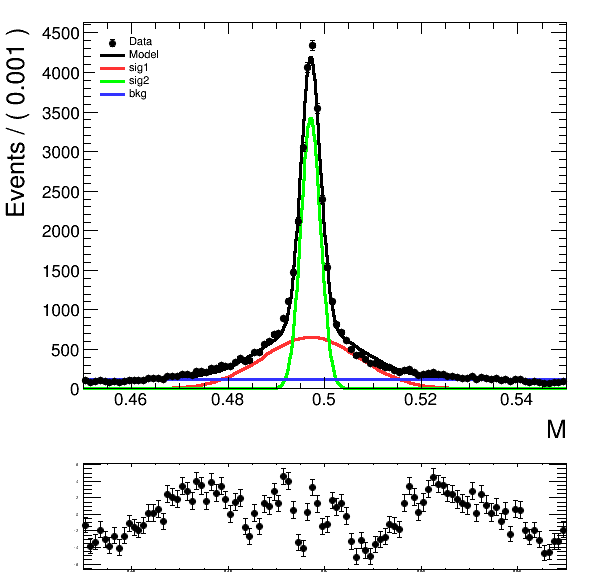
\includegraphics[width=0.85\linewidth]{ksDatamva0.2.png}
	\end{subfigure}
\begin{subfigure}{0.5\linewidth}
	\caption{MC, cut=0.2}
	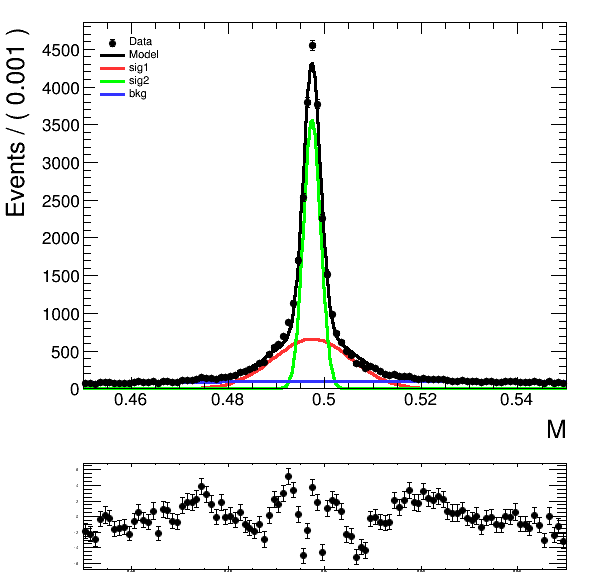
\includegraphics[width=0.85\linewidth]{ksMCmva0.2.png}
\end{subfigure}
\begin{subfigure}{0.5\linewidth}
	\caption{Data, cut=0.4}
	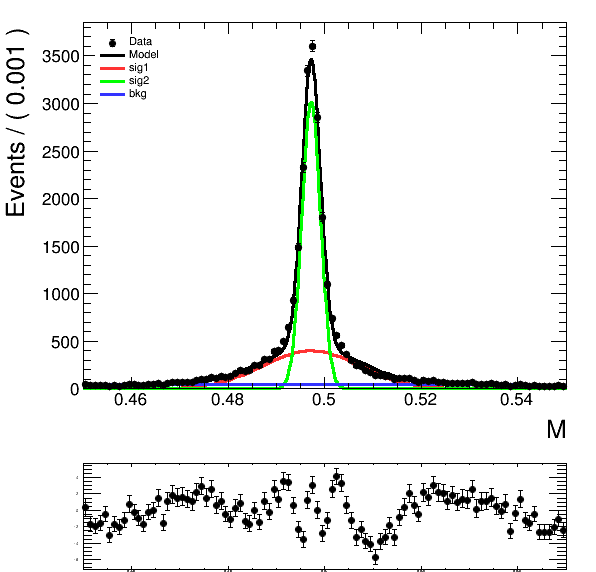
\includegraphics[width=0.85\linewidth]{ksDatamva0.4.png}
\end{subfigure}
\begin{subfigure}{0.5\linewidth}
	\caption{MC, cut=0.4}
	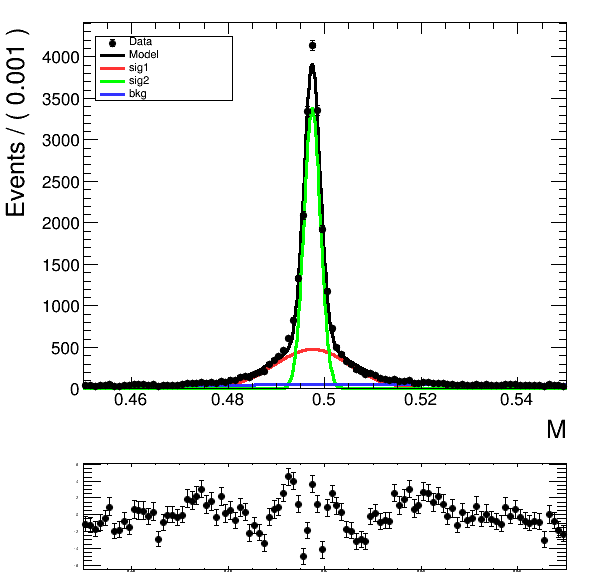
\includegraphics[width=0.85\linewidth]{ksMCmva0.4.png}
\end{subfigure}
\end{figure}


\begin{figure}[H]
	\ContinuedFloat
	\begin{subfigure}{0.5\linewidth}
		\caption{Data, cut=0.5}
		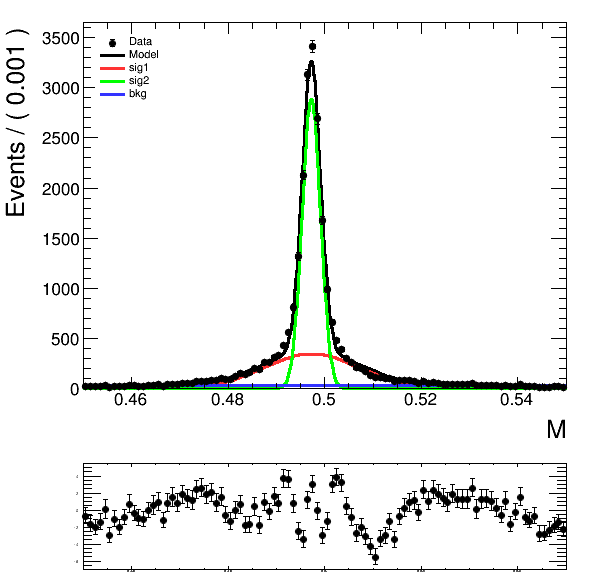
\includegraphics[width=0.85\linewidth]{ksDatamva0.5.png}
	\end{subfigure}
	\begin{subfigure}{0.5\linewidth}
		\caption{MC, cut=0.5}
		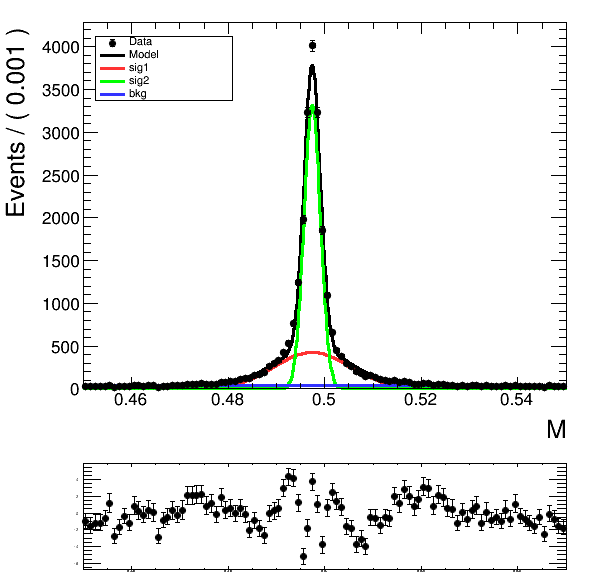
\includegraphics[width=0.85\linewidth]{ksMCmva0.5.png}
	\end{subfigure}
	\begin{subfigure}{0.5\linewidth}
		\caption{Data, cut=0.55}
		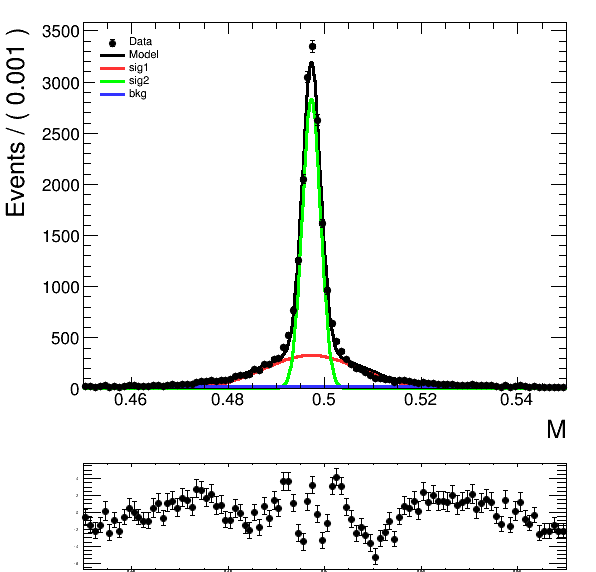
\includegraphics[width=0.85\linewidth]{ksDatamva0.55.png}
	\end{subfigure}
	\begin{subfigure}{0.5\linewidth}
		\caption{MC, cut=0.55}
		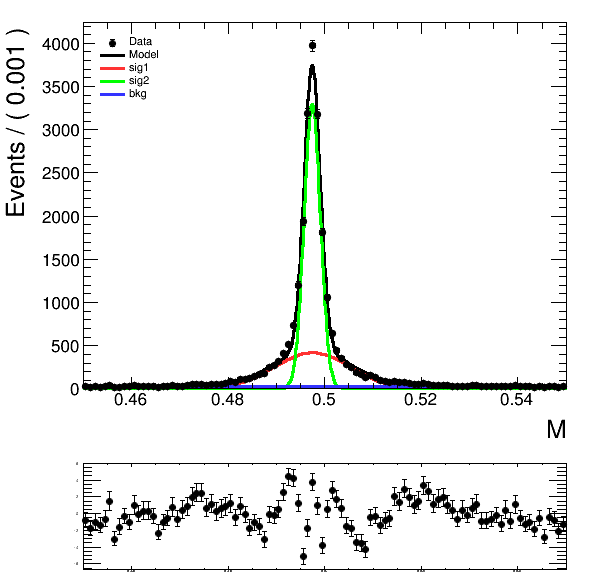
\includegraphics[width=0.85\linewidth]{ksMCmva0.55.png}
	\end{subfigure}
	\begin{subfigure}{0.5\linewidth}
		\caption{Data, cut=0.6}
		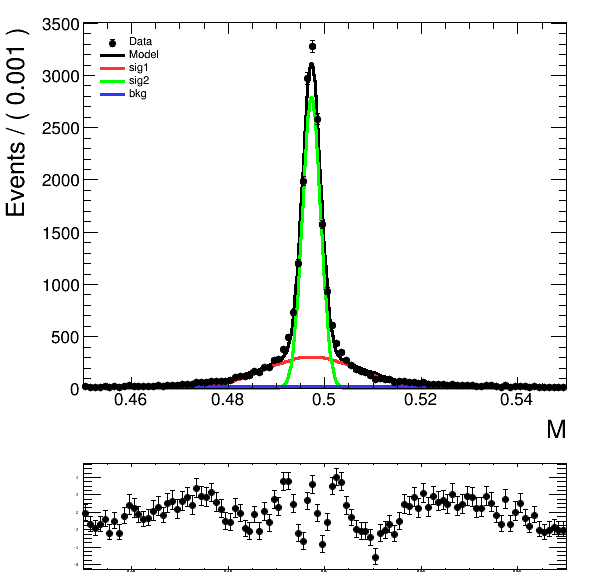
\includegraphics[width=0.85\linewidth]{ksDatamva0.6.png}
	\end{subfigure}
	\begin{subfigure}{0.5\linewidth}
		\caption{MC, cut=0.6}
		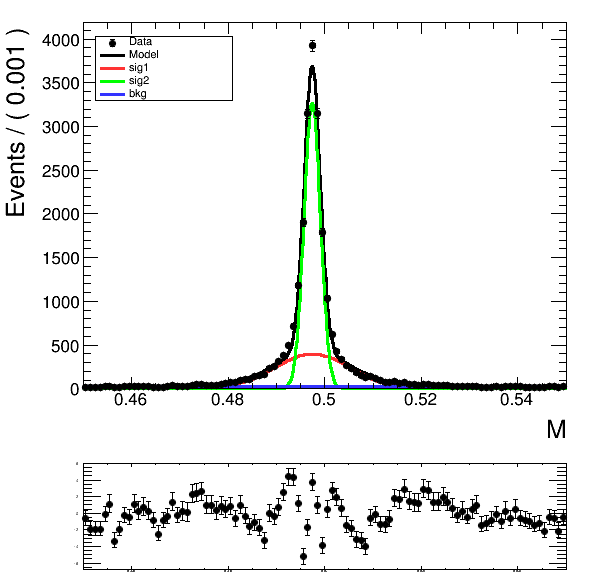
\includegraphics[width=0.85\linewidth]{ksMCmva0.6.png}
	\end{subfigure}
\end{figure}

\begin{figure}[H]
	\ContinuedFloat
	\begin{subfigure}{0.5\linewidth}
		\caption{Data, cut=0.65}
		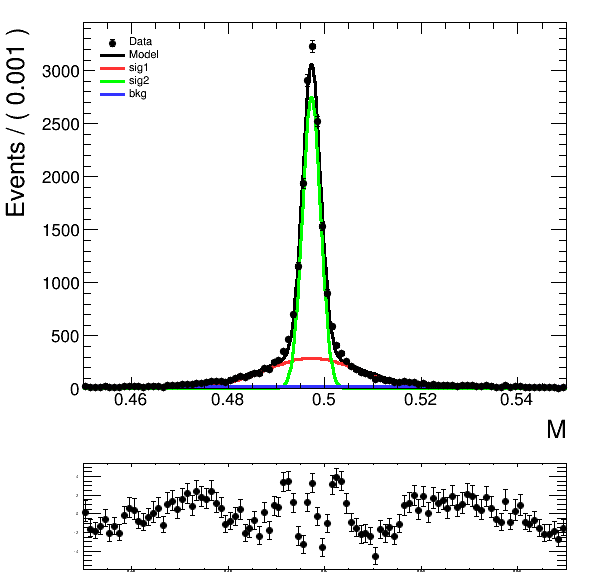
\includegraphics[width=0.85\linewidth]{ksDatamva0.65.png}
	\end{subfigure}
	\begin{subfigure}{0.5\linewidth}
		\caption{MC, cut=0.65}
		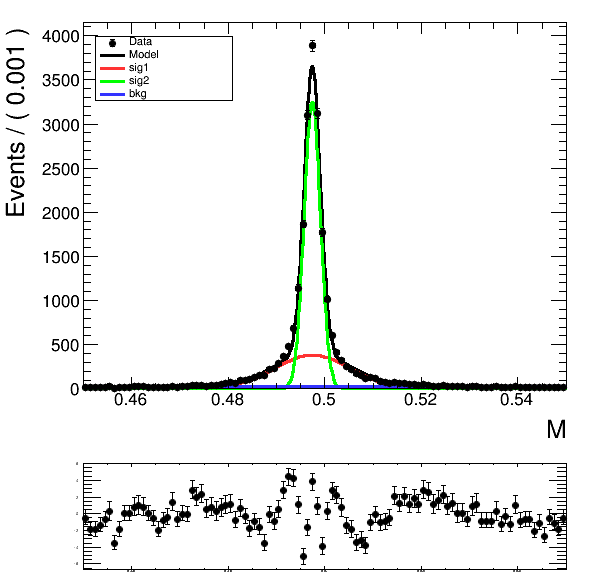
\includegraphics[width=0.85\linewidth]{ksMCmva0.65.png}
	\end{subfigure}
	\begin{subfigure}{0.5\linewidth}
		\caption{Data, cut=0.7}
		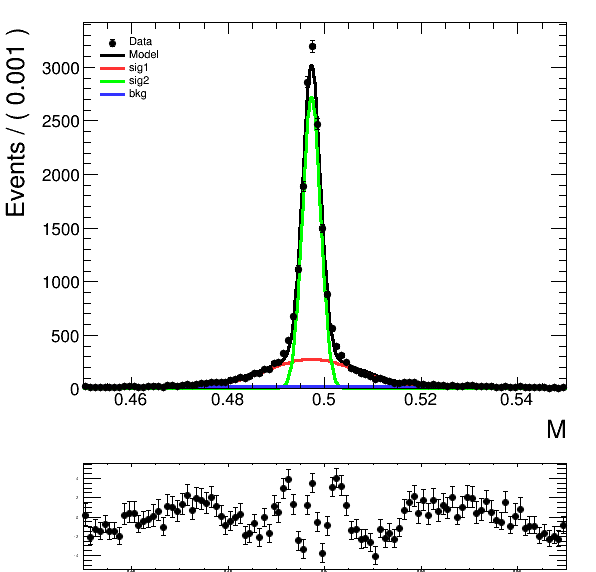
\includegraphics[width=0.85\linewidth]{ksDatamva0.7.png}
	\end{subfigure}
	\begin{subfigure}{0.5\linewidth}
		\caption{MC, cut=0.7}
		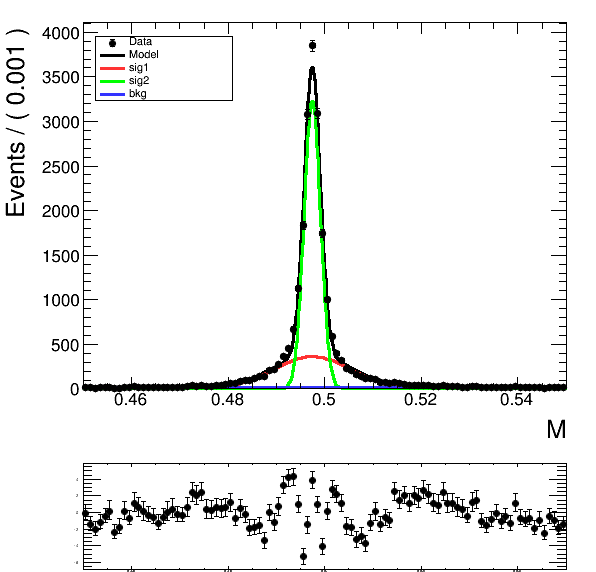
\includegraphics[width=0.85\linewidth]{ksMCmva0.7.png}
	\end{subfigure}
	\begin{subfigure}{0.5\linewidth}
		\caption{Data, cut=0.75}
		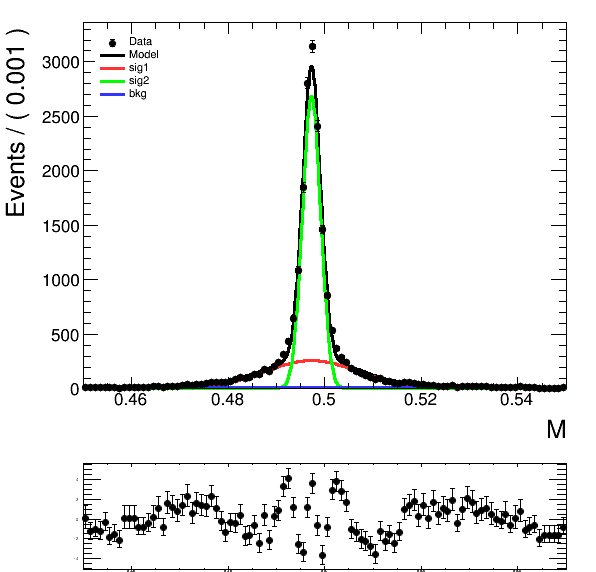
\includegraphics[width=0.85\linewidth]{ksDatamva0.75.png}
	\end{subfigure}
	\begin{subfigure}{0.5\linewidth}
		\caption{MC, cut=0.75}
		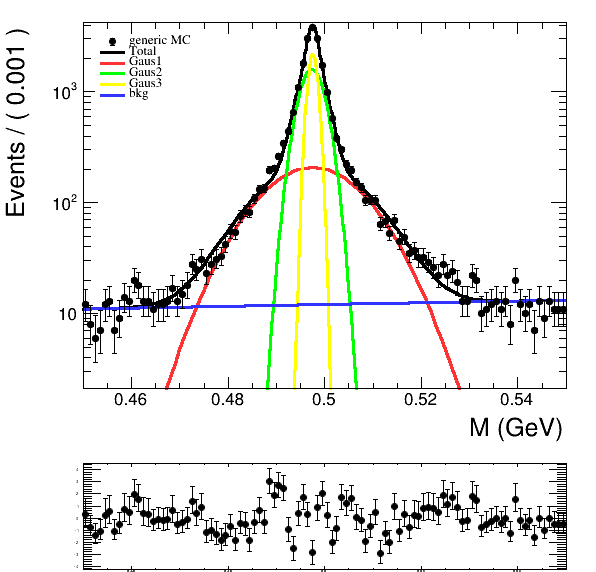
\includegraphics[width=0.85\linewidth]{ksMCmva0.75.png}
	\end{subfigure}
\end{figure}


\begin{figure}[H]
	\ContinuedFloat
	\begin{subfigure}{0.5\linewidth}
		\caption{Data, cut=0.8}
		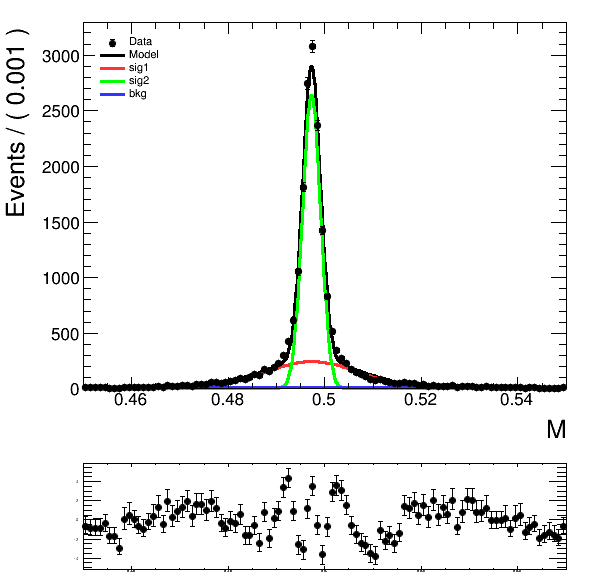
\includegraphics[width=0.85\linewidth]{ksDatamva0.8.png}
	\end{subfigure}
	\begin{subfigure}{0.5\linewidth}
		\caption{MC, cut=0.8}
		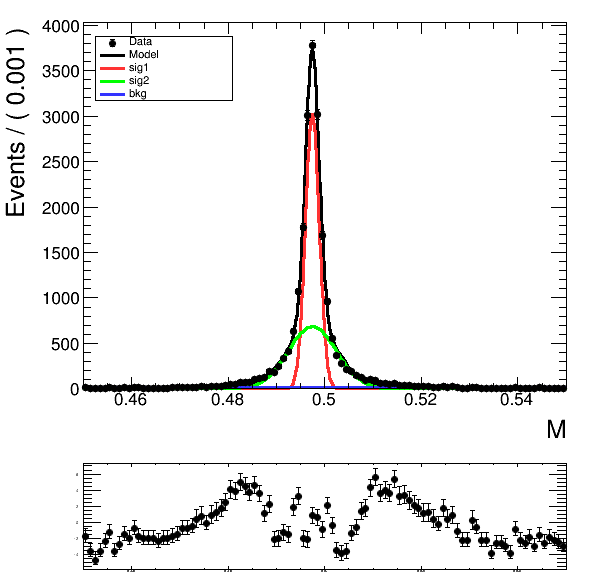
\includegraphics[width=0.85\linewidth]{ksMCmva0.8.png}
	\end{subfigure}
	\begin{subfigure}{0.5\linewidth}
		\caption{Data, cut=0.85}
		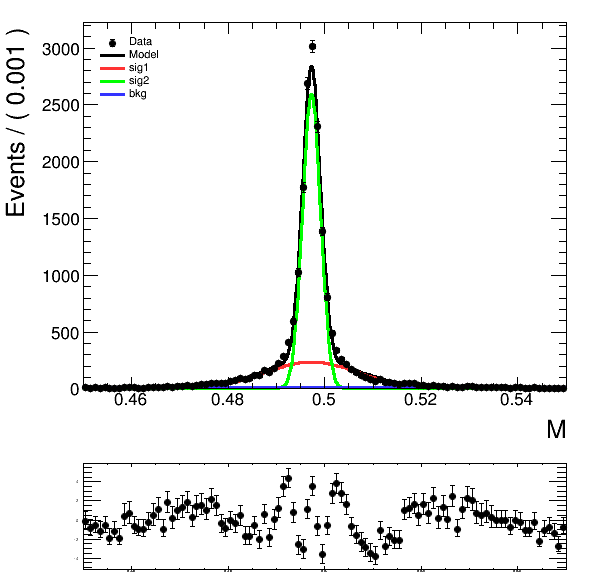
\includegraphics[width=0.85\linewidth]{ksDatamva0.85.png}
	\end{subfigure}
	\begin{subfigure}{0.5\linewidth}
		\caption{MC, cut=0.85}
		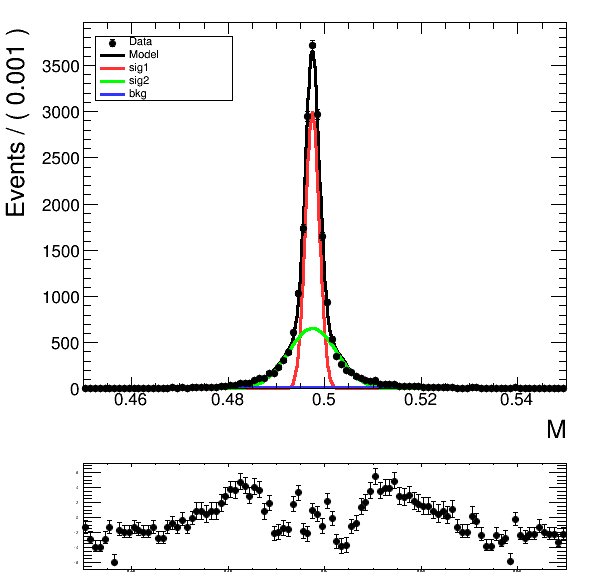
\includegraphics[width=0.85\linewidth]{ksMCmva0.85.png}
	\end{subfigure}
	\begin{subfigure}{0.5\linewidth}
		\caption{Data, cut=0.9}
		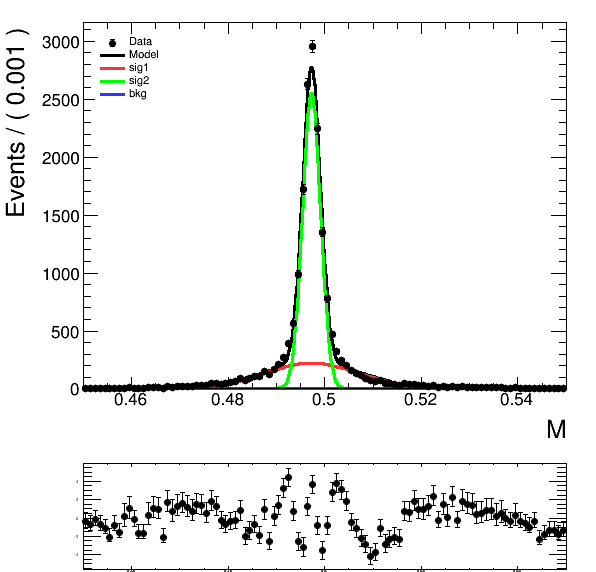
\includegraphics[width=0.85\linewidth]{ksDatamva0.9.png}
	\end{subfigure}
	\begin{subfigure}{0.5\linewidth}
		\caption{MC, cut=0.9}
		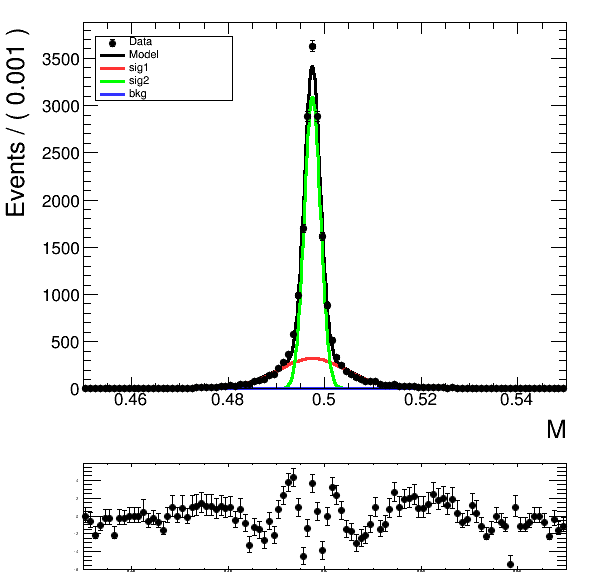
\includegraphics[width=0.85\linewidth]{ksMCmva0.9.png}
	\end{subfigure}
\end{figure}

\begin{figure}[H]
	\ContinuedFloat
	\begin{subfigure}{0.5\linewidth}
		\caption{Data, cut=0.95}
		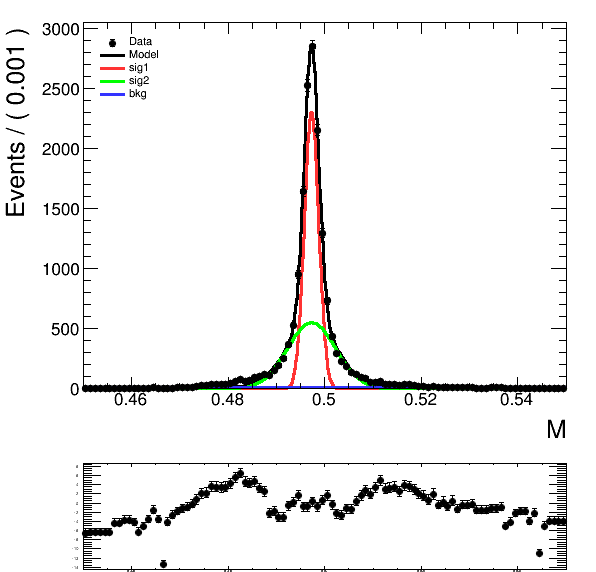
\includegraphics[width=0.85\linewidth]{ksDatamva0.95.png}
	\end{subfigure}
	\begin{subfigure}{0.5\linewidth}
		\caption{MC, cut=0.95}
		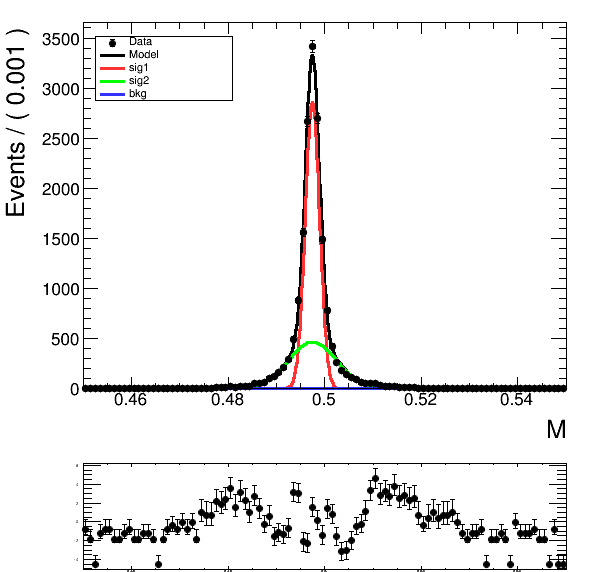
\includegraphics[width=0.85\linewidth]{ksMCmva0.95.png}
	\end{subfigure}
	
\end{figure}
